 
  
\section*{page 4 -- A reconfigurable reinforcement learning system}

{\ }\\

\begin{center}
\scalebox{0.5}{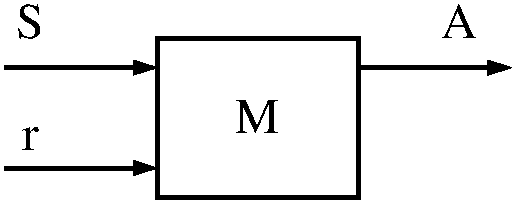
\includegraphics{media/page4diagram.pdf}}
\end{center}

assume a Markov decision process M which can be completely represented as a tuple \( M = \langle S, A, T, R, \pi, \tilde{T}, \tilde{R}\rangle \)\\

\begin{minipage}{5in}
\(S\) -- a set of states $s\in S$ which may be experienced by $M$\\
$A$ -- a set of actions $a\in A$ that may be executed\\
$T$ -- a true transitional probability, $T(s^{\prime}|a,s)$ expressing the probability of executing an action $a$ in state $s$ before ending up in later state $s^{\prime}$.\\
$R$ -- is a reward function which quantifies how desirable a transition $R(s'|a,s)$ is. $R: S\times S\rightarrow \mathbb{R}_{\geq 0}$\\
\textbf{[I changed $\mathbb{R}^{+}$ to $\mathbb{R}_{\geq 0}$ because the former is ambiguous with respect to whether or not 0 is included (online research suggests there is no accepted convention) while the latter is unambiguous.]}\\
$\pi$ -- is an action selection policy, ideally chosen to maximize expected reward, an optimal policy is denoted $\pi^*$. Typically
\begin{equation*}
\pi^*(s) = \argmax_{a}\sum_{s^\prime}\underbrace{R(s^\prime|a,s) T(s'|a,s)+\gamma V(s^\prime)}_{\text{expected reward}}
\end{equation*}
\end{minipage}

\section*{encoding}

To encode the expected reward over all states, typically $Q$-values are kept: \( Q(s,a) \sim \sum R(s^\prime|a,s)T(s^\prime|a,s)+\gamma V(s^\prime) \) and \( Q_{t+1}(s,a) \leftarrow Q_t(s,a)+\alpha \left( R(s^\prime|a,s)-Q_t(s,a)+\gamma\argmax)_{a^\prime} Q(s^\prime,a^\prime) \right) \).

In this paper we rely on a method of extracting dynamic $Q$-values from an encoded transition and reward function $( \tilde{T}, \tilde{R} )$. The motivation for this encoding is that it allows mapping the transition function into multiple spaces, and allows the reward function to be altered. The significance of this finding is covered in \textbf{???} Price wash \textbf{???}.

 
